\documentclass[10pt]{article}
\usepackage[a4paper,margin=17mm]{geometry}
\usepackage{amsmath,amssymb,graphicx,hyperref}
\hypersetup{colorlinks=true,urlcolor=blue}
\setlength{\parindent}{0pt}\setlength{\parskip}{5pt}
\begin{document}
\begin{center}\Large Public-input roots with representative families\\[3pt]
\normalsize Bounded Rust reference, 16 November 2026\\
PCC-20261116-7de4ca; signed standing unverified\end{center}
The reference builds its declared small base from public parameters, then
receives only a target. Discovered roots satisfy the unchanged original
target circuit and independent indexed-row replay. Finite exhaustion and
resource refusal are distinct; no planted labels, scalar or witnesses enter
the query. [pcc:unverified]
\begin{center}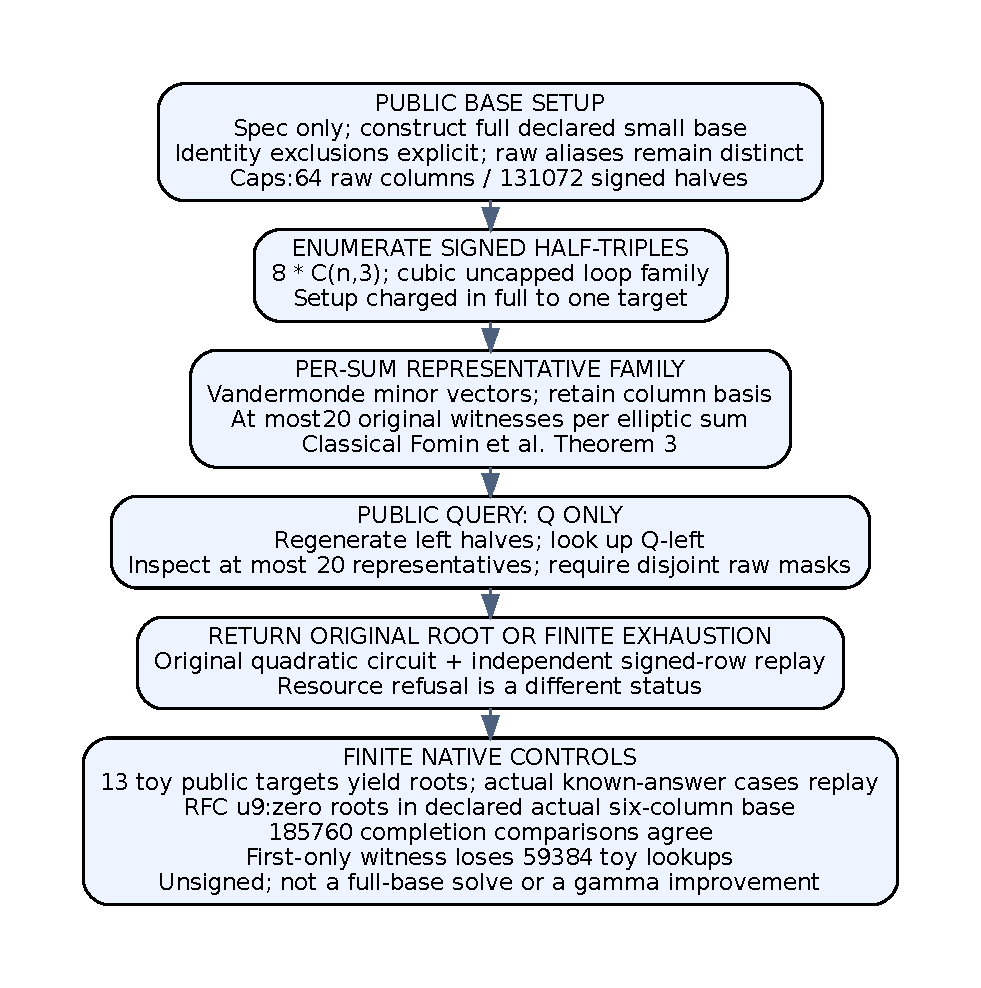
\includegraphics[width=0.98\linewidth,height=155mm,keepaspectratio]{pipeline.pdf}\end{center}
\textbf{Why one witness is insufficient.} A right triple must avoid the
left triple's three raw columns. Selecting only the first triple per elliptic
sum loses 59384 of 160160 toy completion lookups. The first retained example
has half-sum identity, forbidden mask 11, first mask 19 and disjoint valid
mask 2096. This is a lookup failure, not a claim of whole-target solver failure.

\textbf{Classical remedy.} Assign raw label $i$ the Vandermonde vector
$(1,x_i,\ldots,x_i^{2r-1})$, $x_i=i+1$, with prime field size exceeding the
raw count. Store a column basis of its $r$-minor vectors per point sum,
retaining ORIGINAL signed witnesses. Dimension $\binom{2r}{r}\le20$ for
$r\le3$. A nonzero disjoint-completion determinant functional remains
nonzero on one basis witness. This is Fomin et al. Theorem 3, not a new
representative-family theorem or formal compiler proof.
\newpage
\begin{center}\Large Finite coverage and the cubic boundary\end{center}
\begin{center}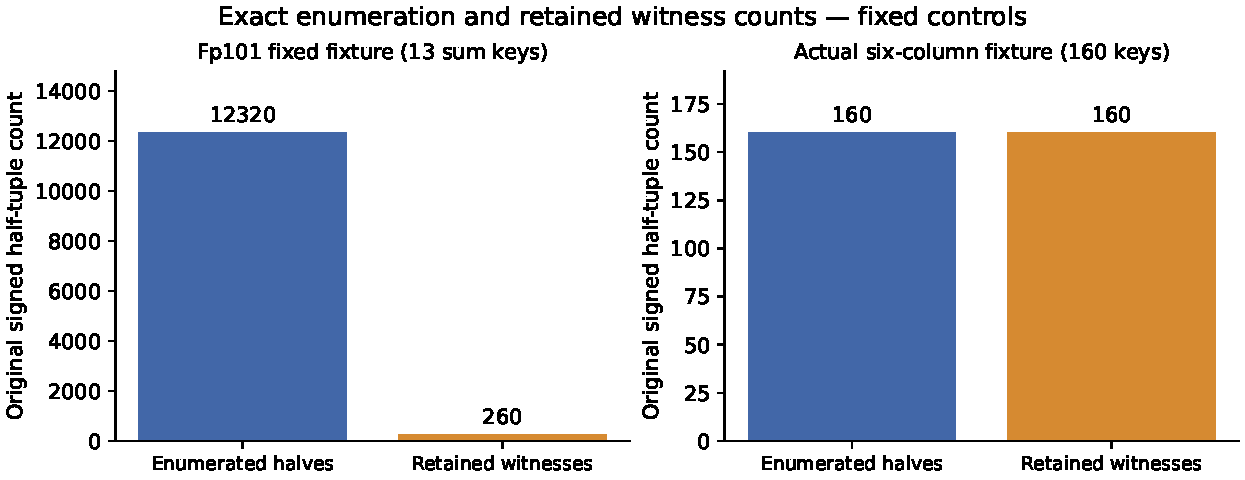
\includegraphics[width=0.99\linewidth]{counts.pdf}\end{center}
These count original witnesses, not RAM bytes or speed. Each representative
also stores up to 20 field coordinates. Diagnostic target reuse establishes
no primary batch performance claim.

\textbf{Toy controls.} Fixed $p=101,A=95,h=(17,12),a=17,q=3,k=8$:
22 retained raw columns after the same two identity exclusions$(1,2),(8,2)$.
All 13 public image targets return six-member roots and replay. All 160160
full-family/representative completion comparisons agree. Max 20 witnesses
per sum; raw image aliases stay separate. [pcc:unverified]

\textbf{Actual bounded fixture.} Actual Curve25519 field/coefficient,
$h_{new}=h_{old}^{213156431}$, $a=60824497,q=1,k=6$:six raw columns,
160 signed triples and160 keys. Arity2/4/6 known-answer targets return
and replay. RFC u9 target exhausts that exact six-column arity6 base;
independent all 64 sign choices also give zero roots. All 25600 compression
queries agree, including 1280 yes/24320 no cases. This is not the huge
actual many-coset base or a general Curve25519 absence result.
[pcc:unverified]

\textbf{Scaling classification.} Shipped caps:64 raw columns/131072
signed halves. Raising caps without replacing the six-member loop still
enumerates $8\binom n3$ triples. Fixed-dimensional algebra and dictionary
factors give cubic construction and up to cubic key storage. Thus this
extension does not meet the subquadratic gate. At the earlier conditional
$n\asymp\ell^{1/6}$ model point, setup alone reaches exponent$1/2$ before
later phases. This rejects that extension, not all index calculus. Charge
setup in full to one target. Selected API events are not total normalized
field work or admitted timing evidence.

\textbf{Reproduction and scope.} Focused release test, fmt/strict Clippy
pass. First lint's needless index loop source/log is retained; enumerate
fix changes no polynomial. The 50-input composite snapshot is the unchanged
43-input v2 dependency archive plus 13808-byte seven-input delta. All hashes,
archive round-trips and seven compiled-in pins match. Full roots/bases and
185760-byte trace (488-byte gzip) are retained. Prior frozen bytes stay
unchanged. [pcc:unverified]

\textbf{Identity.} IDC1hd26c4be98ace1e7d evaluates the standard degree 15
six-column Vandermonde determinant identity over its declared $2^{61}-1$
field in two fixed 32-point streams; a plus-one mutation is refused. This
is not formal or independently signed verification of the solver/instance.

\textbf{Next gate.} A public-input structured solver must avoid explicit
triple enumeration, lift original roots and price setup/failures/yield/all
phases under unchanged route criteria. No benchmark, sampling, paid job,
new solver campaign, full huge-base enumeration or broad library rerun ran.

\textbf{Sources.} Source-linked REPORT.md;
\href{https://arxiv.org/abs/1304.4626}{Fomin et al., arXiv1304.4626v4, sec. 2.5/Theorem 3}; frozen native/RFC sources. KB runtime
unavailable; primary-source fallback. No novelty claim for classical methods.
\end{document}
